\input{../praeambel.tex}

\usepackage[orientation=portrait,size=a0,scale=1.4]{beamerposter}
\usepackage{qrcode}
\usepackage{paracol}
\addbibresource{references.bib}

\usepackage[pscoord]{eso-pic} % The zero point of the coordinate system is the lower left corner of the page (the default).

\setbeamertemplate{blocks}[default] % Remove the shadows and borders of blocks.
\renewcommand{\thempfootnote}{\arabic{mpfootnote}}

\newcommand{\placetextbox}[3]{% \placetextbox{<horizontal pos>}{<vertical pos>}{<stuff>}
  \setbox0=\hbox{#3}% Put <stuff> in a box
  \AddToShipoutPictureFG*{% Add <stuff> to current page foreground
    \put(\LenToUnit{#1\paperwidth},\LenToUnit{#2\paperheight}){\vtop{{\null}\makebox[0pt][c]{#3}}}%
  }%
}%

\author[H. Heyden \and M. Materzok \and N. Pulow \and S. Şimşek]{Henri Heyden \and Mika Materzok \and Nike Pulow \and Senanur Şimşek}
\title{What made music popular in the last 20 years?}

%%%%%%%%%%%%%%%%%%%%%%%%%%%%%%%%%%%%%%%%%%%%%%%%%%%%%%%%%%%%%%%%%%%%%%%%%%%%%%%%%

    % How did song duration change over the years?
    % How did song tempo change over the years?
    % Y What chord-progressions repeat most frequently?
    % Y* Do certain chord(-progressions) dominate specific genres?
    % Y What chords and chord types dominate over the years?
    % How variant are the intervals that are being played?
    % Which words and combinations are the most frequent?
    % How did lyric polarity change? 

\begin{document}
\begin{frame}[t]
\centering
\textit{\textquote{I think music in itself is healing. It's an explosive expression of humanity. It's something we are all touched by. No matter what culture we're from, everyone loves music.}}\\ -- Billy Joel
\begin{columns}
\begin{column}{0.49\textwidth}
    \begin{block}{Motivation} 
        Not only is it interesting to look at popular music from the point of view of musicians aspiring to create the next hit single. Indeed, it is also interesting to analyse recent music since music is an essential part of any culture.
        By analysing popular music one can learn about what the current culture is, how it changed and how it varied.
        In the following, we'll look at the most popular music of the last two decades to answer which musical and lyrical elements we can identify and analyse the change of them.
    \end{block}
    \begin{block}{Harmonic Progressions}
    What main chord repetition should you use to write the perfect song? By scraping chords, identifying their key signature to transpose equal harmonies and looking for repeated patters, we found the most frequently used harmonic progressions of the last 20 years, see figure \ref{fig:harmony}.\\
    The most used harmonic progression (I, VI, III, VII) can for example be played in B-minor with chords Bm, G, D, A, like in Ed Sheeran's \textquote{Shivers}.
    \begin{figure}[hbt!]
        \centering
        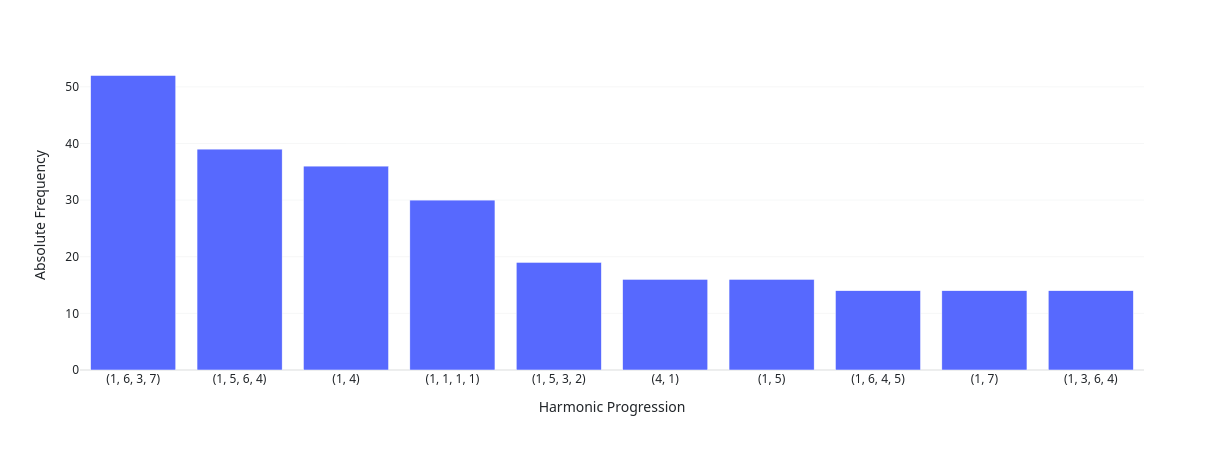
\includegraphics[width=\textwidth]{./figures/2.png}
        \caption{Top ten most used harmonic progressions by absolute frequency.}
        \label{fig:harmony}
    \end{figure} 
    \end{block}
    \begin{block}{Chords}
    Musicians often write songs in the same key they can sing in and therefore use the same chords more often. Most chords in figure \ref{fig:chords} can be played in C-major or A-minor. We can also see that A-minor key is more popular than C-major key, since D and Em work better in A-minor compared to C-major.\footnote[1]{D and Em are roughly the IV and V of A-minor, but the II and III of C-major, which are less important harmonic chords as you can see in figure \ref{fig:harmony}}

    \begin{figure}[hbt!]
        \centering
        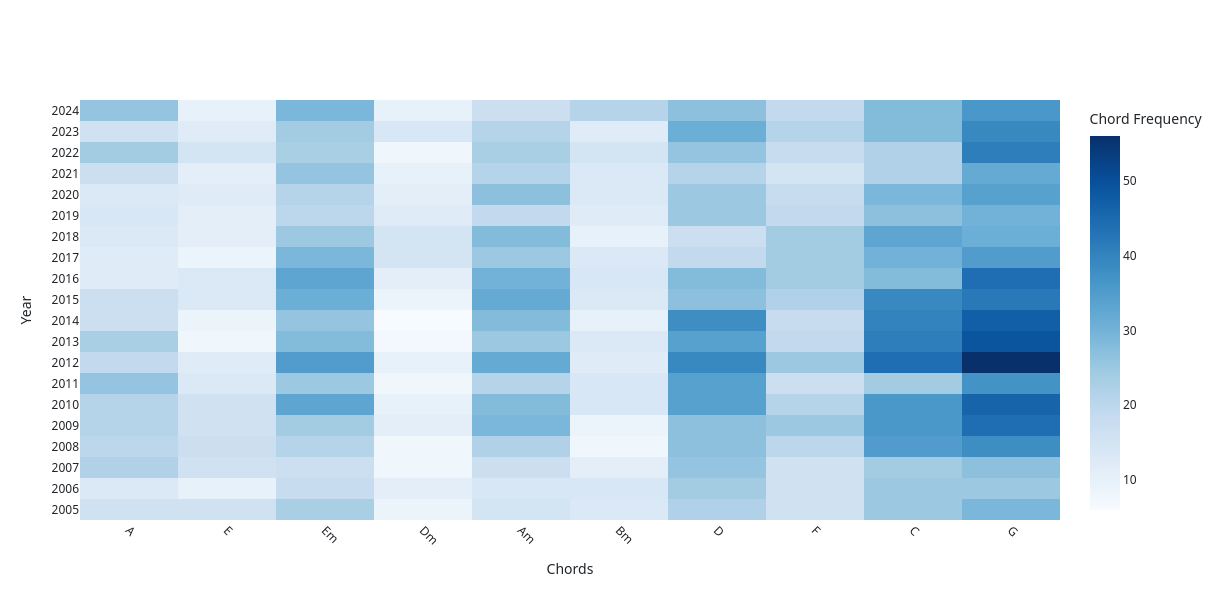
\includegraphics[width=\textwidth]{./figures/1.png}
        \caption{Top ten most used basic chords over the years}
        \label{fig:chords}
    \end{figure}
    
    It shouldn't be surprising, that the most frequent genre in popular music is \textit{pop}-music. \\
    Looking at the top tags of the song we got from LastFM and comparing to the chord frequency, see figure \ref{fig:chordtags}, we can see that \textquote{Hip-Hop} and \textquote{Rap} are also quite popular. We can also identify, that these two genres have the most missing chords which can be explained by their neglection of harmony, since they focus more on rhythm and rime.

    \begin{figure}[hbt!]
        \centering
        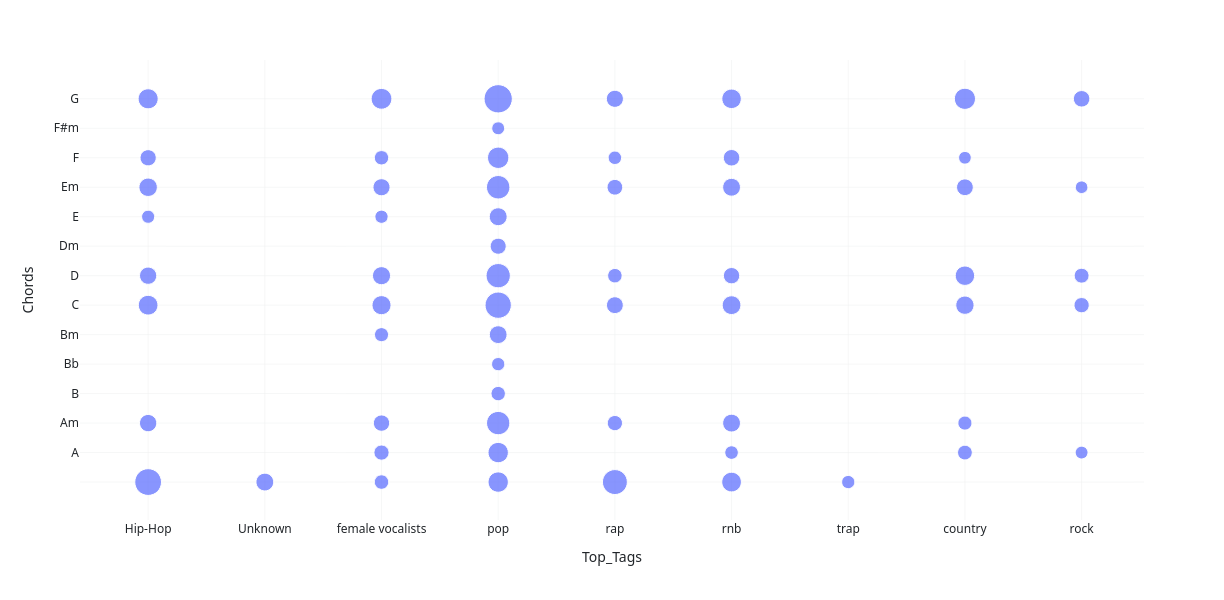
\includegraphics[width=\textwidth]{./figures/5.png}
        \caption{Top ten most frequent genre tags by how often they use some specific chord.}
        \label{fig:chordtags}
    \end{figure}

    \end{block}
    \end{column}
\begin{column}{0.49\textwidth}
    \begin{block}{Song Duration}
    \end{block}

    \begin{block}{Lyrics}
    \end{block}

    \begin{block}{References}
        \printbibliography
    \end{block}
\end{column}
\end{columns}
\placetextbox{0.9}{0.125}{\qrcode[height=9cm]{https://fur-fortnite.onrender.com/}}

%\begin{block}{Titel}
%    Hier ist auch Text
%\end{block}

\end{frame}
\end{document}

